%%%%%%%%%%%%%%%%%%%%%%%%%%%%%%%%%%%%%%%%%%%%%%%%%%%%%%%%%%%%%%%%%
% Dissertacao de Mestrado / Dept Fisica, CFM, UFSC              %
% Lacerda@UFSC - 2013                                           %
%%%%%%%%%%%%%%%%%%%%%%%%%%%%%%%%%%%%%%%%%%%%%%%%%%%%%%%%%%%%%%%%%

%:::::::::::::::::::::::::::::::::::::::::::::::::::::::::::::::%
%                                                               %
%                          Capítulo 3                           %
%                                                               %
%:::::::::::::::::::::::::::::::::::::::::::::::::::::::::::::::%

%***************************************************************%
%                                                               %
%                      PCA e Tomografia PCA                     %
%                                                               %
%***************************************************************%

\chapter{PCA e Tomografia PCA}
\label{sec:PCAeTomoPCA}

De medidas fisiológicas, como pulsação e respiração, até reconhecimento de
padrões em sistemas complexos como reconhecimento facial e criptografia,
passando por compactação de imagem, neurosciência e redução de ruídos em dados,
podemos ver atuação de técnicas de PCA. \ojo Brincando com a própria técnica, o
PCA em si é uma PC de um universo matemático-estatístico.

%***************************************************************% 
%                                                               %
%                              PCA                              %
%                                                               % 
%***************************************************************%

\section{Principal Component Analisys}
\label{sec:PCAeTomoPCA:PCA}

Baseada em encontrar os eixos com maiores variâncias em um conjunto de variáveis
(no nosso caso, fluxos por lambda e por zona), a técnica PCA vem sendo de grande
utilidade quando o assunto é estatística com muitas variáveis. Através de
operações relativamente simples computacionalmente usando álgebra linear, é
feito uma rotação na base de dados original, gerando uma nova base ortonormal
não correlacionada através de um conjunto de autovalores e autovetores.

Existem diversas formas de se calcular essa base final. A prova matemática que
você pode obter essa base é feita através de multiplicadores de Lagrange,
calculando os autovetores e autovalores ($\mathbf{e}{}_k$ e $\lambda_k$) que
maximizam o valor de $\mathbf{e}{}_k^T \cdot \mathbf{C}{}_{cov} \cdot
\mathbf{e}{}_k$ (ver Eq. \ref{eq:PCA:covMatrix}) sujeito a restrição de que um
autovetor deve ser ortogonal a qualquer outro da base ($\mathbf{e}{}_i^T
\mathbf{e}{}_j = 0$) e que todos devem ser normalizados ($\mathbf{e}{}_i^T
\mathbf{e}{}_i = 1$) \citep[][p. 5-6]{JolliffePCA1986}. Para esse cálculo usamos
a biblioteca científica \texttt{SciPy}\footnote{\url{http://scipy.org/}}
(\ref{fig:PCA:covMatrix}), que encontra os autovetores e autovalores da matriz
de correlação.

\subsection{PCA das galáxias do CALIFA}

Conforme a Seção \ref{sec:CALePyC:PyCASSO} vimos que o cubo de espectros das
galáxias do CALIFA estão acessíveis no PyCASSO separados por zonas. Os espectros
observados estão armazenados em forma de uma matriz $(n \times m)$ com $n$ zonas
e $m$ comprimentos de onda (\texttt{f\_obs}\footnote{No PyCASSO está amostrado
de forma transposta ($\lambda \times z$) a usada.} no PyCASSO). No PCA que
estamos aplicando, cada espectro de uma zona pode ser represtado como um ponto
num espaço $m-dimensional$. Encontramos então quais são os eixos mais
significativos desse espaço em relação à variância. 

\begin{equation}
    \label{eq:PCA:fluxMatrix}
    \textbf{F}{}_{z \lambda} = \left[
    \begin{array}{ccccc}
        f_{z_0 \lambda_0} & f_{z_0 \lambda_1} & f_{z_0 \lambda_2} & ... & f_{z_0 \lambda_m} \\
        f_{z_1 \lambda_0} & f_{z_1 \lambda_1} & f_{z_1 \lambda_2} & ... & f_{z_1 \lambda_m} \\
        f_{z_2 \lambda_0} & f_{z_2 \lambda_1} & f_{z_2 \lambda_2} & ... & f_{z_2 \lambda_m} \\
        ...               & ...               & ...               & ... & ...               \\
        f_{z_n \lambda_0} & f_{z_n \lambda_1} & f_{z_n \lambda_2} & ... & f_{z_n \lambda_m} 
    \end{array} 
    \right]
\end{equation}

Calculamos então o espectro médio de uma galáxia através da equação $\langle
\textbf{F}{}_\lambda \rangle = (1 / n) \sum_{i=0}^{n} f_{z_i}{}_{\lambda}$ e
então subtraímos a média de todos os espectros ($\textbf{I}{}_{z \lambda} =
\textbf{F}{}_{z \lambda} - \langle \textbf{F}{}_\lambda \rangle$) para o cálculo
da matriz de covariâncias usando um conjunto de dados com média zero. Vemos que
a matriz de covariância possui dimensão $\lambda \times \lambda$. 

\begin{equation}
	\label{eq:PCA:covMatrix}
	\mathbf{C}{}_{cov} = \frac{[\mathbf{I}{}_{z \lambda}]^T \cdot \mathbf{I}{}_{z
	\lambda}}{n - 1}
\end{equation}

Agora calculamos os autovalores e autovetores da matriz de covariância. Neste
trabalho usamos o nome autoespectro para designar esses autovetores pois são de
uma matriz de covariâncias entre espectros de cada zona. Então ordenamos-os
decrescentemente pelo valor de seus autovalores. Os autoespectros são as PCs e
os autovalores as variâncias. Isso feito, temos então o que necessitamos para
iniciar o cálculo do Tomograma PCA.

\begin{figure}
\begin{python}
# Carregar arquivo FITS com os dados.
from pycasso import fitsQ3DataCube
K = fitsQ3DataCube('K0277_synthesis_suffix.fits')

# Calcular o espectro medio de uma galaxia. 
# K.f_obs tem dimensao (lambda, zona), portanto, 
# fazemos o espectro medio de todas as zonas.
f_obs_mean__l = K.f_obs.mean(axis = 1)

# Subtraimos a media
I_obs__zl = K.f_obs.transpose() - f_obs_mean__l

# Calcular a matrix de convariancia
import scipy as sp
n = K.N_zone
dot_product = sp.dot(I_obs__zl.transpose(), I_obs__zl)
covMat__ll = dot_product / (n - 1.0)   

# Calcular os autovalores e autovetores
w, e = linalg.eigh(covMat__ll)

# Ordenar os autovetores decrescentemente pelo seu autovalor
S = sp.argsort(w)[::-1]
eigval = W[S]
eigvect = e[:, S]
 
\end{python}
	\caption[Exemplo de cálculo de PCA usando o PyCASSO e SciPy] {Cálculo do
	procedimento completo de PCA para os espectros observados de uma galáxia do
	CALIFA usando o PyCASSO e a biblioteca científica de Python chamada
	\texttt{SciPy}. No final do código temos eigval e eigvect que são os
	autovalores e autovetores ordenados em forma decrescente.}
	\label{fig:PCA:covMatrix}
\end{figure}

Muitas figuras de PCs e suas utilizações e diferenças nos pré-processamentos
serão mostradas nos Capítulos \ref{sec:UsoPCA} e \ref{sec:result}, juntamente
com a Tomografia PCA e as comparações com os parâmetros físicos da sintese de
populações estelar.

%***************************************************************%
%                                                               %
%                        Tomografia PCA                         %
%                                                               %
%***************************************************************%

\section{Tomografia PCA}
\label{sec:PCAeTomoPCA:TomoPCA}

Na técnica de PCA procuramos os autoespectros (PCs) da matriz de correlação,
ordenados pela variância, formam uma base ($\mathbf{E}{}_{\lambda k}$) onde 
podemos projetar os nossos dados através da transformação:

\begin{equation}
	\label{eq:TomoPCA:tomogram2D}
	\mathbf{T}{}_{z k} = \mathbf{I}{}_{z \lambda} \cdot \mathbf{E}{}_{\lambda k}
\end{equation}

Projetamos nossa matriz de observáveis com a média subtraida ($\mathbf{I}{}_{z
\lambda}$) na base das PCs ($\mathbf{E}{}_{\lambda k}$). Na posse dessa nova
matriz transformada e de um mapa que leve de zona para uma par de coordenada ($z
\to (x, y)$), podemos montar assim uma imagem. Cada imagem funciona como uma
``fatia'' de um cubo de dados expandido na nova base, assim formando a
Tomografia PCA\footnote{\url{http://www.astro.iag.usp.br/~pcatomography/}},
criada e assim batizada por \citet{Steiner2009}, que em seu artigo faz um
paralelo com fatias de um espaço tridimensional (tomograma do corpo humano, por
exemplo) ou no espaço de velocidades (Tomografia Doppler). Cada ``fatia'' possui
um autoespectro relacionado que, em conjunto, trazem novas perspectivas e ideias
para a interpretação de ambos. A passagem de coordenadas $z \to (x, y)$ está
exemplificada na Figura \ref{fig:mapaIdade} através da função de
\texttt{zoneToYX} dentro do PyCASSO.

\subsection{Evidências de linhas largas}

No artigo citado anteriormente, através do estudo dos autoespectros, e suas
respectivas imagens, da galáxia LINER ({\em Low Ionizations Nuclear
Emission-line Region}) NGC 4736, foram encontradas evidências de {\em broad
lines} nas regiões nucleares da galáxia. Quando temos uma fonte que é capaz de
produzir linhas largas no espectro é sinal da existência de um SMBH ({\em Super
Massive Black Hole}). \citet{CidFernandes2004} mostra que a subtração bem
detalhada das populações estelares nos espectros ajuda a encontrar linhas largas
mais fracas em Seyferts-II, que são aquelas que possuem linhas estreitas,
ajudando assim em na classificação desses objetos como tipo I ou II. O PCA,
juntamente com a Tomografia PCA, fazem esse papel da subtração das populações
estelares sem haver nenhuma parametrização.

Foram estudados os primeiros 8 autoespectros escolhidos através de um {\em scree
test} (\ref{fig:TomoPCA:scree}), no qual se verifica a variância de cada PC e
toma-se as mais relevantes. O autoespectro com mais variância (no artigo tratado
com E1) possui $99.74\%$ da variância e reproduz comportamento do gás e da
população estelar somados (Figura \ref{fig:TomoPCA:eigspec1}). O segundo
contribui com $0.088\%$ para a variância e tem um claro padrão de rotação, tanto
nas linhas do autoespectro quanto na imagem da tomografia (Figura
\ref{fig:TomoPCA:eigspec2}). Mas é no terceiro ($0.032\%$ da variância) que
mostra evidências de uma emissão larga de \Halpha (Figura
\ref{fig:TomoPCA:eigspec3}). Essa assinatura e uma evidência tipica de objetos
com um AGN associado a um SMBH (Seyfert-I).

Com isso em mãos podemos estudar a Tomografia PCA nas galáxias do CALIFA. Temos
disponíveis várias galáxias com os cubos de dados COMBO e aplicaremos essa
técnica às galáxias presentes na Tabela \ref{tab:pixelZones} no Capítulo
\ref{sec:result}.

\begin{figure}
    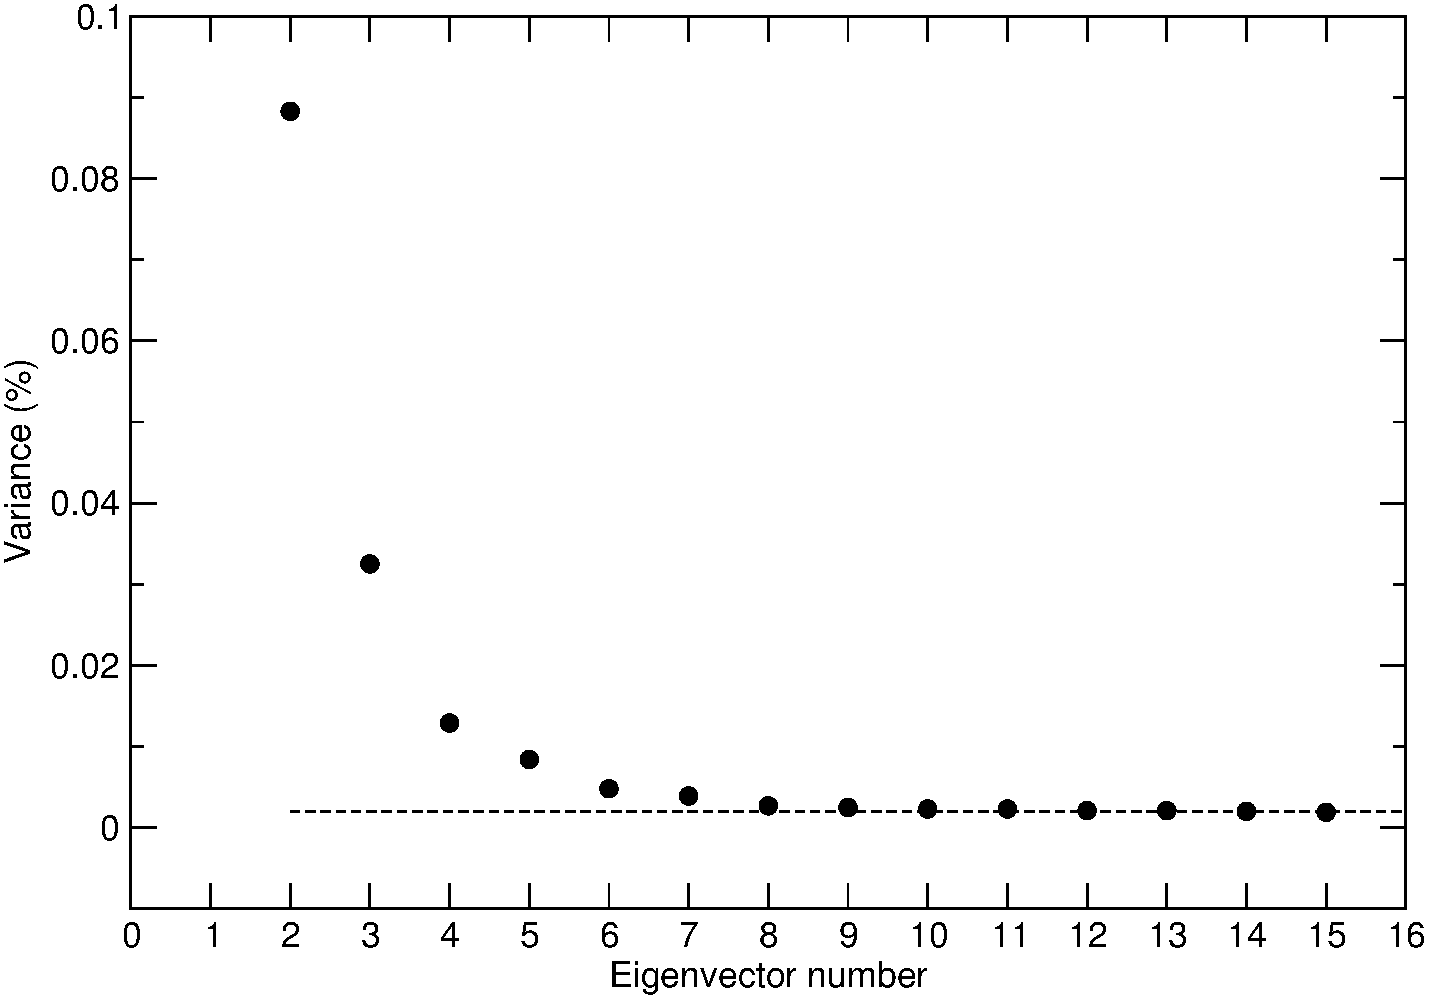
\includegraphics[width=0.7\textwidth]{figuras/figSteiner2009fig1.pdf}
    \caption[{\em Scree test} na galáxia NGC 4736.]
    {Scree test das primeiras 16 PCs do cubo de espectros da região
    central da galáxia NGC 4736. Retirado de \citet[][fig. 1]{Steiner2009}.}
    \label{fig:TomoPCA:scree}
\end{figure}

\begin{figure}
    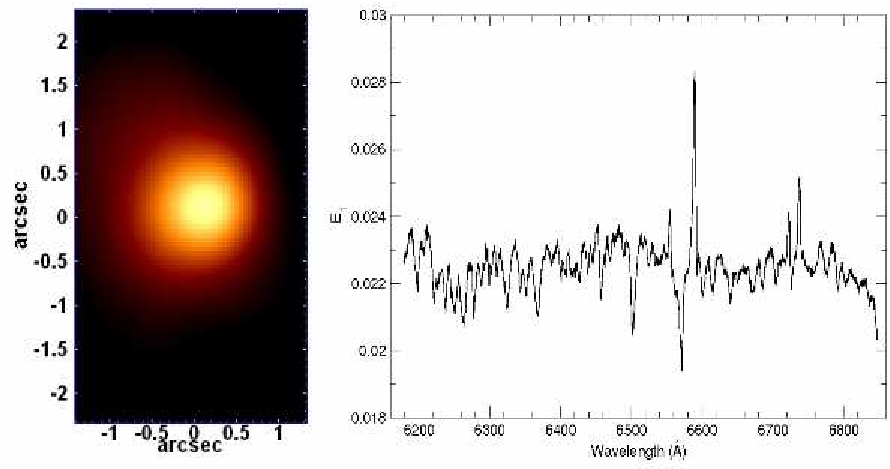
\includegraphics[width=0.9\textwidth]{figuras/figSteiner2009figA1.pdf}
    \caption[Tomograma e autoespectro 1 da galáxia NGC 4736.]
    {Autoespectro 1 e seu respectivo tomograma. Retirado de \citet[][fig.
    A1]{Steiner2009}.}
    \label{fig:TomoPCA:eigspec1}
\end{figure}

\begin{figure}
    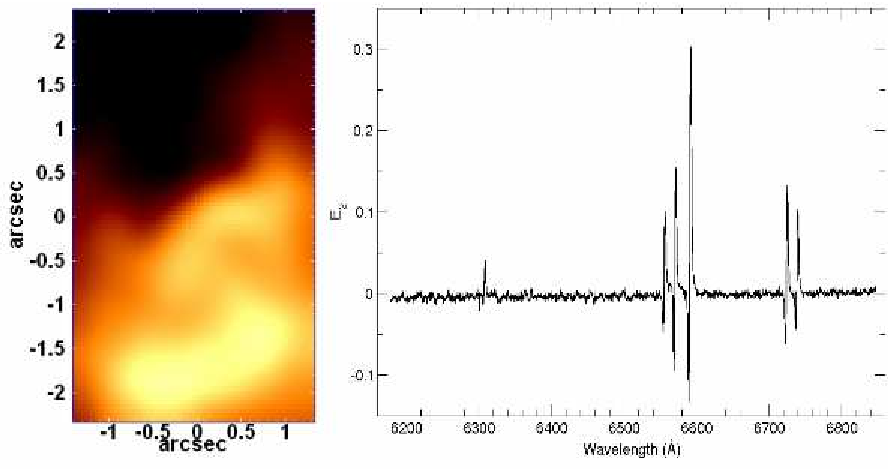
\includegraphics[width=0.9\textwidth]{figuras/figSteiner2009figA2.pdf}
    \caption[Tomograma e autoespectro 2 da galáxia NGC 4736.]
    {Autoespectro 2 e seu respectivo tomograma. Retirado de \citet[][fig.
    A2]{Steiner2009}.}
    \label{fig:TomoPCA:eigspec2}
\end{figure}

\begin{figure}
    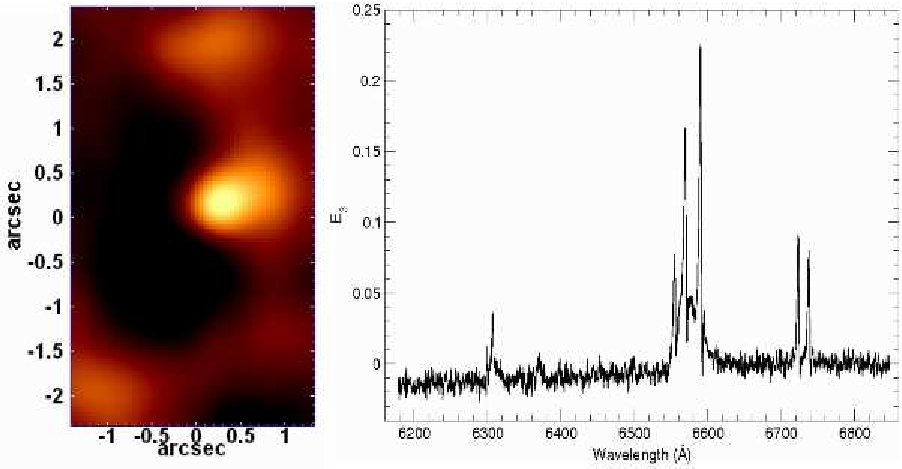
\includegraphics[width=0.9\textwidth]{figuras/figSteiner2009figA3.pdf}
    \caption[Tomograma e autoespectro 3 da galáxia NGC 4736.]
    {Autoespectro 2 e seu respectivo tomograma. Retirado de \citet[][fig.
    A3]{Steiner2009}.}
    \label{fig:TomoPCA:eigspec3}
\end{figure}

%% End of this chapter
